\documentclass[../../dissertation.tex]{subfiles}
\begin{document}

In the quantum case, the walker is a system whose position on a
discretely numbered line, is described by a vector $\ket{x}$ in Hilbert space.
The next position of the system will depend, in part, of a unitary operator,
which can be viewed as a quantum coin.
%TODO: \textcolor{red}{O operador unitário não é somente da moeda, precisa
%falar do espaço do caminhante também}
The analogy is, if the coin is tossed and rolls "heads", for example, the
system transitions to position $\ket{x+1}$, otherwise it advances to
$\ket{x-1}$. From a physical perspective, this coin can be the spin of an
electron or the chirality of a particle, for example, and the outcome of
measuring these properties decides whether the walker moves left or right. The
coin is a unitary operator defined as
%TODO: Decidir se ponho as letras ou explico de outra maneira.
\begin{equation}
	\begin{cases}
		C\ket{0} = a\ket{0} + b\ket{1}\\
		C\ket{1} = c\ket{0} + d\ket{1},
	\end{cases}
\end{equation}
where $a$, $b$, $c$ and $d$ are the amplitudes associated with each outcome of
the coin toss. One of the most commonly used coins is the unbiased coin, also
known as the Hadamard operator
\begin{equation}
	H = \begin{pmatrix} 
		a & c\\
		b & d
	    \end{pmatrix}
	    =\frac{1}{\sqrt{2}} \begin{pmatrix}
			    		1 & 1\\
					1 & -1
	   		       \end{pmatrix},
\end{equation}
which will be the one used in this example.\par 

The Hilbert space of the system is $\mathscr{H} = \mathscr{H}_{C} \otimes
\mathscr{H}_{P}$, where $\mathscr{H}_{C}$ is the two-dimensional Hilbert space
associated with the coin and $\mathscr{H}_P$ is the Hilbert space of the
walker.\par The transition from $\ket{x}$ to either $\ket{x+1}$ or $\ket{x-1}$
must be described by a unitary operator, the \textit{shift operator} 
%TODO: \textcolor{red}{precisa descrever a moeda também e como ela funciona no
%unitário e acredito que as equações estejam trocadas}
\begin{equation}
	\begin{cases}
		\mathcal{S} \ket{0}\ket{x} = \ket{0}\ket{x+1}\\
		\mathcal{S} \ket{1}\ket{x} = \ket{1}\ket{x-1},
	\end{cases}
\end{equation}
that can also be described by
\begin{equation}
	S = \ket{0}\bra{0} \otimes \sum_{x=-\infty}^{x=\infty} \ket{x+1}\bra{x} + \ket{1}\bra{1}\otimes \sum_{x=-\infty}^{x=\infty} \ket{x-1}\bra{x}.
	\label{eq:coinedShiftOperator}
\end{equation}
It follows that the operator that describes the dynamics of the quantum walk
will be given by 
\begin{equation}
	U = S(C\otimes I) = S(H\otimes I). 
	\label{eq:coinedUnmarkedOperator}
\end{equation}\par
Consider a quantum system located at $\ket{x = 0}$ with coin state $\ket{0}$,
for $t=0$. It's state will be described by
\begin{equation}
	\ket{\psi(0)} = \ket{0}\ket{x=0}.
	\label{eq:coinedQWInitCond0}
\end{equation}
After $t$ steps 
\begin{equation}
	\ket{\psi(t)}=U^{t}\ket{\psi(0)},
\end{equation}
more explicitly
\begin{equation}
	\ket{\psi(0)}\xrightarrow[]{\text{$U$}}\ket{\psi(1)}\xrightarrow[]{\text{$U$}}\ket{\psi(2)}\xrightarrow[]{\text{$U$}} (...) \xrightarrow[]{\text{$U$}}\ket{\psi(t)}.
\end{equation}\par
In summary, the coined quantum walk algorithm consists of applying the coin
operator followed by the shift operator a certain number of times. Iterating
this twice, evolves the system to the following states
%TODO: \textcolor{red}{seria bom especificar que é na moeda, ou até mesmo dizer que o quantum walk consiste da aplicação da moeda e logo em seguida o shift}
\begin{equation}
	\ket{\psi(1)} = \frac{\ket{0}\ket{x=-1}+\ket{1}\ket{x=1}}{\sqrt{2}}
\end{equation}
\begin{equation}
	\ket{\psi(2)} = \frac{\ket{0}\ket{x=-2}+\ket{1}\ket{x=0}+\ket{0}\ket{x=0}-\ket{1}\ket{x=2}}{2}
\end{equation}
If one were to measure the system after the first application of $\mathcal{U}$,
it would be expected to see the walker at $x=1$ with probability $P(x) =
\frac{1}{2}$, and at $x=-1$ with $P(x) = \frac{1}{2}$. Measure the
system $t$ times, after each application of $\mathcal{U}$, and the result is a
binomial probability distribution similar to the one in figure
\ref{fig:MultClassicalWalk72180450}. The conclusion is that repetitive
measurement of a coined quantum walk system reduces to the classical case,
which means that any desired quantum behavior is lost. \par

It is possible, however, to make use of the quantum correlations between
different positions to generate constructive or destructive interference, by
applying the Hadamard and shift operators successively without intermediary
measurements.  The consequences of interference between states become very
apparent after only 3 iterations 
\begin{equation}
	\ket{\psi(3)} = \frac{\ket{1}\ket{x=-3}-\ket{0}\ket{x=-1}+2(\ket{0}+\ket{1})\ket{x=1}+\ket{0}\ket{x=3}}{2\sqrt{2}}\label{eq:12}.
\end{equation}

Even though an unbiased coin was used, this state is not symmetric around the origin and the probability distributions will not be centered in the origin. Moreover, \cite{REN1} shows that the standard deviation will be
\begin{equation}
	\sigma(t) \approx 0.54t .
\end{equation}
This means that the standard deviation for the coined quantum walk grows
linearly in time, unlike the classical case which grows with $\sqrt{t}$, as was
seen in equation \eqref{eq:classicalWalkDeviation}. The implication is that the
quantum walk displays \textit{ballistic} behaviour, as is reviewed in
\cite{andraca2012}. This behaviour is usually defined in the context of a
moving free particle with unit velocity in a single direction, which is
expected to be found at $x=t$ after $t$ steps. The velocity of a walker in a
Hadamard quantum walk is approximately half of the free particle example, which
is still a quadratic improvement over the classical random walk. Figure
\ref{fig:coinedClassicalStdDev} shows the comparison between the evolution of
the classical and the quantum standard deviation.
\begin{figure}[!h]
	\centering
	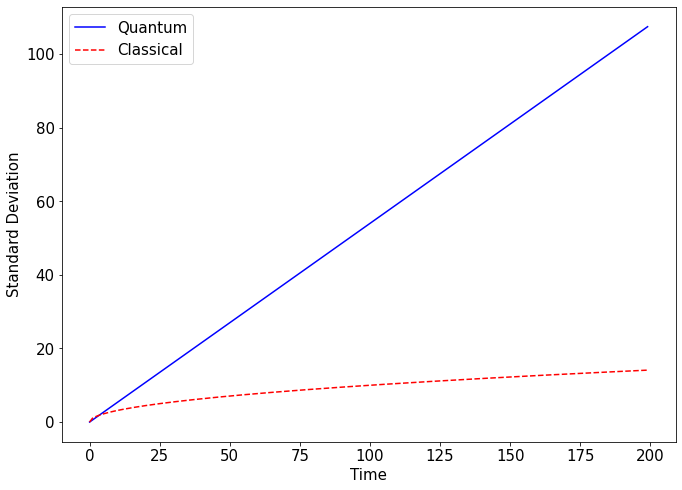
\includegraphics[scale=0.40]{img/CoinedQuantumWalk/coinedClassicalStdDev.png}
	\caption{Standard deviation after $200$ steps for the quantum walk in blue, and the classical random walk in red.} 
	\label{fig:coinedClassicalStdDev}
\end{figure}\par
This quadratic gain implies exponentially faster hitting times in certain
graphs, as shown by \cite{childs2002}, meaning improvements to problems that
require transversing graphs. \cite{ambainis2003} also shows advantages of the
coined quantum walk model in element distinctness problems, and
\cite{childs2004} show advantages in spatial search problems, which will be
studied in a later chapter.\par
%TODO: \textcolor{red}{Bom, faltou dizer qual o desvio padrão da quantum walk que é $t$ e esse $\sqrt{t}$ é da clássica. Precisa justificar com alguma referência também}\par
%The quantum walk is said to be \textit{ballistic} since its standard deviation is proportional to $t$ \cite{andraca2012} meaning exponentially faster hitting times in certain graphs \cite{childs2002,fahri98} which can be advantageous in problems that involve visiting certain vertices in a graph. There are also studies that show that a quantum walk may have advantages in element distinctness \cite{ambainis2003} and spatial search \cite{childs2004} problems. 
%TODO: \textcolor{red}{talvez esse parágrafo deva subir, porque você fala de desvio padrão muito antes}
\begin{figure}[!h]
	\centering
	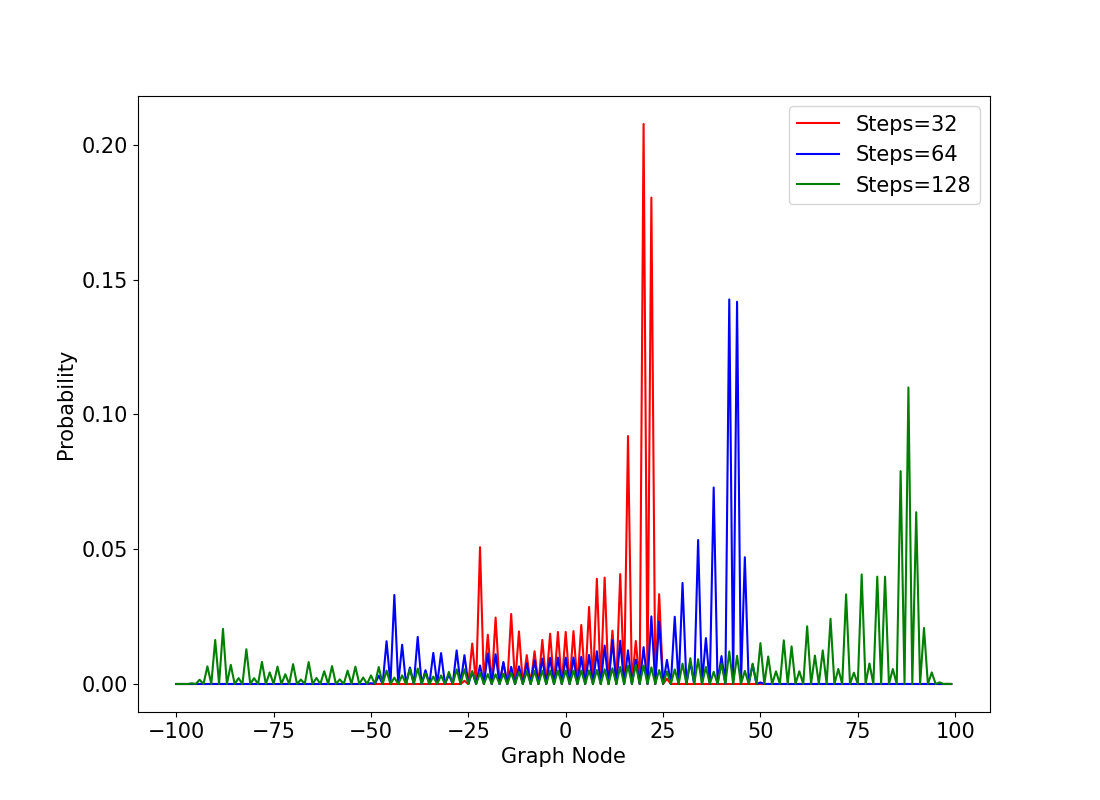
\includegraphics[scale=0.40]{img/CoinedQuantumWalk/CoinedMultiple_psi0_3264128.png}
	\caption{Probability distribution for the coined quantum walk on a line, after $32$, $64$ and $128$ steps, with initial condition $\ket{\psi(0)}=\ket{0}\ket{x=0}$ and the Hadamard coin.} 
	\label{fig:coinedQWDist0}
\end{figure}
In order to study this distribution, a simulation of the coined quantum walk
was coded in \textit{Python}. Figure \ref{fig:coinedQWDist0} is the result of
using the Hadamard coin and the initial condition in equation
\ref{eq:coinedQWInitCond0}, for varying numbers of steps. Analyzing the plot,
it is noticeable that the distributions are asymmetric. The probability of
finding the walker on the right-hand side is much larger than on the left, with
a peak around $x \approx \frac{t}{\sqrt{2}}$. Regardless of number of steps,
this peak is always present (albeit in varying positions), which is to say that
the walker can always be found moving in a uniform fashion away from the
origin, consistent with ballistic behaviour.\par 
%TODO: \textcolor{red}{agora penso que um grafo sobre desvio padrão seria bom para ilustrar, porque o desvio padrão foi muito comentado ao longo do texto}\par

Another interesting case study is to find if this behaviour is preserved for a
symmetric distribution around the origin. For this purpose, one must first
understand where the asymmetry comes from.
\begin{figure}[!h]
	\centering
	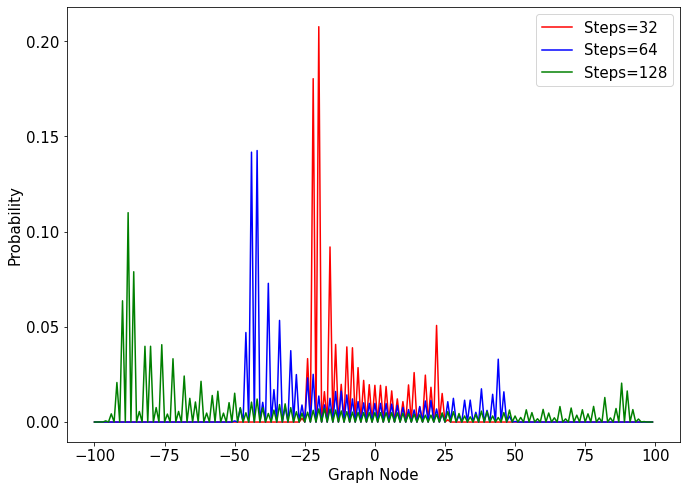
\includegraphics[scale=0.40]{img/CoinedQuantumWalk/CoinedMultiple_psi1_3264128.png}
	\caption{Probability distribution for the coined quantum walk on a line, after $32$, $64$ and $128$ steps, with initial condition $\ket{\psi(0)}=-\ket{1}\ket{x=0}$ and the Hadamard coin.} 
	\label{fig:coinedQWDist1}
\end{figure}
The Hadamard operator flips the sign of state $\ket{1}$, hence more terms are
cancelled when the coin state is $\ket{1}$. Since $\ket{0}$ was defined to
induce movement to the right, the result is as shown in
\ref{fig:coinedQWDist0}. Following this logic, it would be expected that an
initial condition 
%TODO: \textcolor{red}{cuidado com a notação embaixo dos kets, e esse sinal negativo é necessário? acredito que não.} Pagina 30 do renato, perceber melhor o sinal.
\begin{equation}
	\ket{\psi(0)} = \ket{1}\ket{x=0},
	\label{eq:coinedQWInitCond1}
\end{equation}
would result in more cancellations when the coin state is $\ket{0}$, thus the
walker would be more likely found in the left-hand side of the graph. This is
indeed what happens, as figure \ref{fig:coinedQWDist1} is a mirror image of
figure \ref{fig:coinedQWDist0}. The walker still moves away from the origin
with ballistic behavior, but in the opposite direction. The peaks behave in a
similar fashion, being instead found at $x \approx -\frac{t}{\sqrt{2}}$.\par

In order to obtain a symmetrical distribution, one must superpose the state in
equation \eqref{eq:coinedQWInitCond0} with the state in equation
\ref{eq:coinedQWInitCond1}. However, in order to not cancel terms before the
calculation of the probability distribution, one must multiply state $\ket{1}$
with the imaginary unit, $i$ 
%TODO:\textcolor{red}{o sinal pode ser justificado apenas aqui}
%TODO: Justificar que o sinal de i pode ser +-.
\begin{equation}
	\ket{\psi(0)} = \frac{\ket{0}+i\ket{1}}{\sqrt{2}}\ket{x=0}.
	\label{eq:12}
\end{equation}
\begin{figure}[!ht]
	\centering
	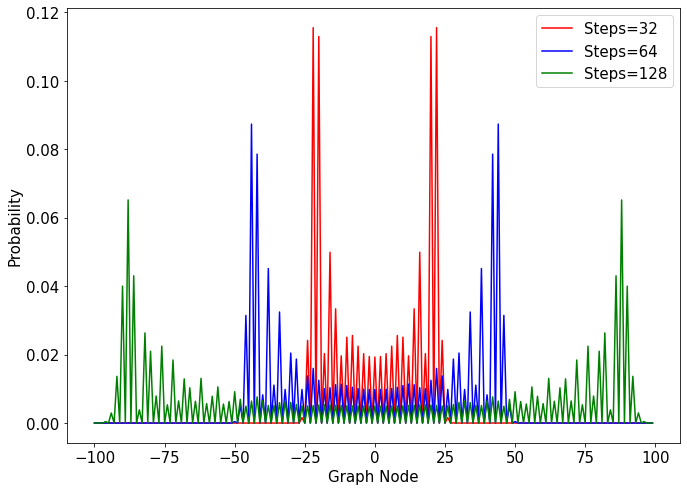
\includegraphics[scale=0.40]{img/CoinedQuantumWalk/CoinedMultiple_psi01_3264128}
	\caption{Probability distribution for the coined quantum walk on a line, after $32$, $64$ and $128$ steps, with initial condition $\ket{\psi(0)}=\frac{\ket{0}-i\ket{1}}{\sqrt{2}}\ket{x=0}$ and the Hadamard coin.} 
	\label{fig:coinedQWDist01}
\end{figure}
This works because the entries of the Hadamard operator are real numbers. Terms
with the imaginary unit will not cancel out with terms without it, thus the
walk can proceed to both left and right, as it is shown in figure
\ref{fig:coinedQWDist01}.  The probability distribution is now symmetric and it
is spread over the range $[-\frac{t}{\sqrt{2}},-\frac{t}{\sqrt{2}}]$ with peaks
around $x \approx \pm \frac{t}{\sqrt{2}}$. This means that if the position of
the walker was measured at the end, it would be equally probable to find him
either in the left side or the right side of the graph which is not possible
in a classical diffusive motion.\par 

All of the previous examples are in sharp contrast with the classical random
walk distribution in figure \ref{fig:MultClassicalWalk72180450}. There, the maximum
probability is reached at $x=0$ since there are approximately equal steps in
both directions.  Furthermore, the further the vertex is away from the origin,
the less likely the walker is to be found there. However, in the quantum case,
the walker is more likely to be found away from the origin as the number of
steps increases.  More specifically, the walk spreads quadratically faster than
the classical counterpart.\par

%TODO: Melhorar o preview das proximas seccoes.
This is but one model of a quantum random walk. As it will be seen in further
sections, there are other approaches to creating both discrete and continuous
quantum walk models that do not use a coin. 

\end{document}
